\documentclass[12pt]{report}

\usepackage{times}
\usepackage[onehalfspacing]{setspace}
\usepackage[a4paper,includehead=true,top=30mm,headsep=10mm,bottom=40mm,textwidth=150mm]{geometry}
\usepackage{fancyhdr}
\usepackage{titlesec}
\usepackage{acro}
\usepackage{enumitem}
\usepackage{hyperref}
\usepackage{graphicx}
\usepackage[font={small,stretch=0.8},labelfont=bf,labelsep=space]{caption}
\usepackage[backend=biber,sorting=nyt,sortcites=true]{biblatex}
\usepackage{amsmath}

\usepackage{lipsum}  % For inserting bogus content.

% ------------------------------------------------------------------------------

% Header customization. For a comprehensive description of the following code,
% check: 'Page layout in LaTeX', by Piet van Oostrum.
\pagestyle{fancy}

% The \chapter command automatically switches to the plain page style, ignoring
% the page style currently in effect. To customize such pages, you must redefine
% the plain pagestyle.
\fancypagestyle{plain}{%
  \fancyhf{}                          % Get rid of headers and footers...
  \fancyfoot[C]{\textbf{\thepage}}    % ...except the center.
  \renewcommand{\footrulewidth}{0pt}  % Also get rid of lines.
  \renewcommand{\headrulewidth}{0pt}}

% Redefine \sectionmark.
\renewcommand{\sectionmark}[1]{\markright{\thesection\ #1}}

% Non-chapter pages are customized by using commands that target specific parts
% of the header/footer. For example, \fancyhead[L] modifies the left portion of
% the header.
\fancyhf{}
\fancyhead[L]{\small\textbf{\leftmark}}  % \leftmark contains the chapter name.
\fancyhead[R]{\small\textbf{\thepage}}
\renewcommand{\headrulewidth}{1pt}

% ------------------------------------------------------------------------------

% Change the size of chapter headings...
\titleformat{\chapter}[display]
{\normalfont\Large\bfseries}{\chaptertitlename\ \thechapter}{25pt}{\LARGE}

% ...and the spacing between chapter and name.
\titlespacing*{\chapter}{0pt}{60pt}{50pt}

% Change the size of section headings.
\titleformat{\section}
{\normalfont\large\bfseries}{\thesection}{1em}{}

% ------------------------------------------------------------------------------

% Define a new list style...
\newlist{acronyms}{description}{1}
\setlist[acronyms]{format=\textnormal,labelindent=7.5mm,labelwidth=25mm,noitemsep}

% ...and attach it to 'acrostyle'.
\DeclareAcroListStyle{acrostyle}{list}{list=acronyms}

% Set the style for the list and the format for the acronyms' first expansion.
\acsetup{list-style=acrostyle,first-long-format=\em\lowercase}

% Acronyms.
\DeclareAcronym{aslw}{short=ASLW,long=A Super Long Word}
                % Look for abbreviations in 'abbrvs.tex'.
\graphicspath{{images/}}      % Look for figures and images in 'images/'.
\addbibresource{refs.bib}     % Look for the bibliography in 'refs.bib'.

\def\chapterautorefname{Ch.}  % Show referenced chapters as 'Ch. XX'.

% ------------------------------------------------------------------------------

\begin{document}

\begin{titlepage}
  \centering
  \vspace*{1in}
  \begin{Large}\bfseries
    Title of the Thesis goes here\par
  \end{Large}
  \vspace{1in}
  \begin{large}
    Name goes here\par
  \end{large}
  \vfill
  A Thesis submitted for the degree of...\par
  \vspace{0.5in}
  Name of the institution goes here\par
  \vspace{0.5in}
  Date goes here\par
\end{titlepage}
 % Add the title page.

% ------------------------------------------------------------------------------

% Front matter.
\cleardoublepage%
\pagenumbering{roman}

\chapter*{Abstract\markboth{Abstract}{}}

\lipsum[1-2]
         % Add the abstract.
\chapter*{Acknowledgments\markboth{Acknowledgments}{}}

\lipsum[3-4]
  % Add the acknowledgments.
\tableofcontents                  % Add the ToC.
\chapter*{List of Abbreviations\markboth{List of Abbreviations}{}}

\addcontentsline{toc}{chapter}{List of Abbreviations}

\printacronyms[heading=none]
   % Add the LoA.

% ------------------------------------------------------------------------------

% Main matter.
\cleardoublepage%
\pagenumbering{arabic}

% Show the current section name in the header of chapters.
\fancyhead[L]{\small\textbf{\rightmark}}

% Add chapters.
\chapter{A Chapter}

\lipsum[5]

\section{A section}

This is a reference~\cite{ref1} \lipsum[6-7]

\section{Another section}

This is \ac{aslw} \lipsum[8]

\begin{figure}[htbp]  % h: here, t: top, b: bottom, p: put on special page.
  \centering
  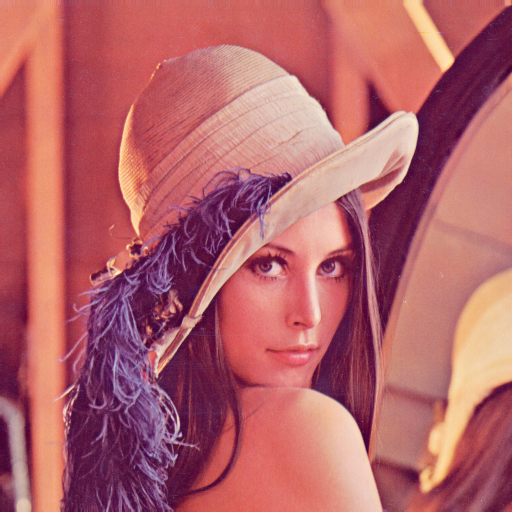
\includegraphics[width=0.5\textwidth]{lenna.png}
  \caption{Caption goes here.}
\end{figure}

\lipsum[9-11]

\chapter{Another Chapter}

\section{Yet another section}

This is another reference~\cite{ref2} \lipsum[12-13]


% Show the name of the bibliography in the header.
\defbibheading{biblio}[\bibname]{
  \chapter*{#1}
  \markboth{#1}{#1}
  \addcontentsline{toc}{chapter}{#1}
}

% Add the bibliography.
\printbibliography[heading=biblio]

\end{document}